\chapter{Concept design}
This chapter defines the global restraints on the concepts and presents an overview of the different concepts.

\section{Global restraints}
This section describes the global restraints on the concepts, as stated in the system requirements. 
\subsection{Myocardium}
\label{sec:myocardium}
To ensure compatibility to the clinical software, \textit{4DM}, the myocardium's HLA and VLA must have the shape of a horseshoe and the SA must have the shape of a circle. 4DM requires these shapes to determine the contours and consequently determine the myocardial flow.
\subsection{Modality}
\label{sec:modality}
The main research question is based around the, relatively new in the Netherlands, D-SPECT's dynamic scanning. Therefore, the modality is bounded to the D-SPECT. As mentioned in section \ref{sec:concept_oper}, the D-SPECT is a suitable choice for myocardial perfusion imaging but still requires validation, which is the goal of the PhD research of which this project is part of.
\subsection{Tracer}
\label{sec:tracer}
The tracer and injection method are fixed due to clinical, 4DM, and dynamic scanning requirements. The clinical (and D-SPECT) protocol use \textsuperscript{99m}Tc (Technetium) Tetrofosmin for myocardial perfusion imaging. To ensure proper dynamic scanning results, the tracer must be injected with a pump. The pump can repeatedly inject tracer with identical volumes and injection speeds.
\subsection{Flow Type}
\label{sec:flowType}
Based on background information on the 4DM software, a decision has been made to use a non-pulsatile flow. The D-SPECT uses gated measurements such that images are extracted at the same point in time of the cardiac cycle. Furthermore, initial experiments with the D-SPECT, with non-pulsatile flow, have been performed on February 5, 2019. The prototype set-up from the individual project, with a dialysis tube, was placed in the D-SPECT and the TAC was extracted. This curve showed proper similarity to TACs extracted from patients.
\section{Design categories}
Each concept is based on the mind map shown in appendix \ref{app:mind_map}. The following sections describe each aspect of the five main categories, respectively:
\begin{itemize}[noitemsep]
	\item Myocardium,
	\item Modality,
	\item Design,
	\item Tracer, and
	\item Flow.
\end{itemize}
\subsection{Myocardium}
The myocardium has two subcategories, the shape and the model.
\subsection*{Shape}
As described in section \ref{sec:myocardium}, the shape of the myocardium is especially important for the 4DM software since it searches for the contours of the left ventricle's walls. Therefore, the shape of the myocardium is fixed (as per system requirements):

\begin{center}
\begin{minipage}{0.3\textwidth}
\begin{itemize}
	\item \ac{VLA}: Horseshoe (figure.
	\item \ac{HLA}: Horseshoe.
	\item \ac{SA}: circle.
\end{itemize}
\end{minipage}%
\begin{minipage}{0.3\textwidth}
\begin{figure}[H]
	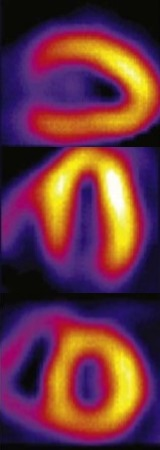
\includegraphics[height=5cm]{./images/stacked_shapes.jpg}
	\caption{Left ventricle's myocardial shapes: VLA, HLA, SA, respectively \citep{niwaz2015pres}}
	\label{fig:ventr_shape}
\end{figure}
\end{minipage}
\end{center}
\subsection*{Model}
\rrot{this section, depending on 4dm}.
The 4DM software offers different segment models in addition to the full 17-segment model, i.e. ...... The goal is to develop a phantom with 17 segments. However, 4DM's ability to downscale to a fewer-segment model, provides the opportunity for a more simplified first prototype.
\subsection{Modality}
As described in section \ref{sec:modality}, the modality is fixed to the D-SPECT's dynamic scanning.
\subsection{Design}
The phantom can be designed in three different ways: using a 1-, 2-, or 4-chamber design. The 1-chamber design simulates only the left ventricle with the myocardium. The 2-chamber design simulates either the left and right ventricles, or the left atrium and ventricle. The other combinations, i.e. left ventricle and right atrium, and any combination without the left ventricle, do not hold any additional benefits. The 4-chamber design contains all heart chambers to simulate the flow as physiological as possible. A 3-chamber design is not considered since it has no physiological structure nor does it have an added benefit over a 1- or 2-chamber design.
\subsection{Tracer}
As described in section \ref{sec:tracer}, the tracer protocol is fixed.
\subsection{Flow}
\subsection*{Generator}
The flow in the phantom can be realised by a various of methods (or combinations thereof):
\begin{itemize} [noitemsep]
	\item Peristaltic pump,
	\item Gear pump,
	\item Air pressure,
	\item Dedicated myocardial generator,
	\item Branching aorta.
\end{itemize}
\subsection*{Supply}
The supply can be realised by a direct connection to the tap (water mains) or via a reservoir which can be filled directly from the tap or manually, e.g. using watering pots. In case of a closed circuit, see section \ref{sec:config}, the reservoir can be filled by the outflow of the phantom.

The D-SPECT room only has a regular indoor faucet making it more difficult to reliably connect to, and the faucet need to be constantly opened and closed between experiments to prevent overflowing. Therefore, although more manual labour, it is safer to manually fill an input reservoir using, for example, watering pots.
\subsection*{Disposal}
Proper disposal of contaminated water (nuclear tracer) will be a vital. Any fluid, or materials, that come into contact with the radioactive tracer, needs to be isolated for a period of multiple days. Spills should be avoided at all costs. Waste fluid can be stored in reservoirs, wheeled (closed) containers, or wheelie bins (Dutch "Kliko"). In case of a closed circuit, see section \ref{sec:config}, the outgoing flow can be directed to the input reservoir.

In any case, the contaminated fluid must be collected in a closed container due to safety reasons. The size of the closed container will depend on the configuration and on the physical limitations at the ZGT.

\subsection*{Configuration}
\label{sec:config}
The flow set-up can be designed in either a closed circuit or open circuit. The closed circuit characterises itself by having no continuous disposal flow, see figure \ref{fig:closed_circ}. The perfusate from the reservoir must be renewed between experiments. The optional filter can extract, if possible, the tracer from the perfusate such that first pass perfusion is realised. Otherwise, the tracer is recirculated which causes the bolus to disappear. An alternative is an open circuit, see figure \ref{fig:open_circ}, which guarantees first pass perfusion due to the absence of any form of recirculation.
\begin{minipage}{0.5\textwidth}
\begin{figure}[H]
	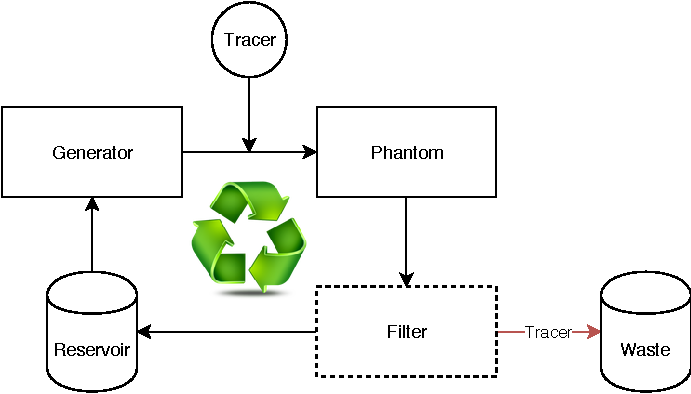
\includegraphics[width=\linewidth]{./images/concept_design_closedCircuit.pdf}
	\caption{Closed circuit schematic design}
	\label{fig:closed_circ}
\end{figure}
\end{minipage}%
\begin{minipage}{0.5\textwidth}
\begin{figure}[H]
	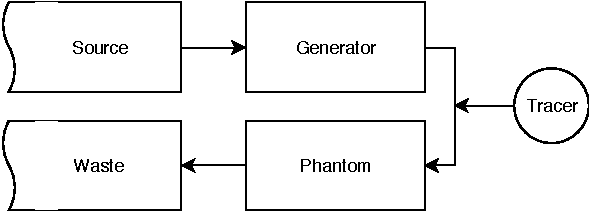
\includegraphics[width=\linewidth]{./images/concept_design_openCircuit.pdf}
	\caption{Open circuit schematic design}
	\label{fig:open_circ}
\end{figure}
\end{minipage}
\subsection*{Type}
As described in section \ref{sec:flowType}, the flow type is fixed.
\subsection*{Perfusate}
Two types of perfusate can be chosen from: water and blood-mimicking fluid (BMF). Water is most practical since it is available in a steady supply. However, BMF is of the same viscosity as human blood allowing for better simulations. However, it needs to be made before any experiments can be performed and in such quantity that it will not run out. In an open circuit configuration, see section \ref{sec:config}, BMF will rapidly be put into the waste collection making it very costly and would therefore be more suitable in a closed circuit configuration.

\section{Concepts}
\begin{table}[H]
\caption{Concept overview}
\raggedright
\begin{tabular}{ll|lll|}
										& 				& \multicolumn{1}{c}{Concept 1} & \multicolumn{1}{c}{Concept 2} &\multicolumn{1}{c}{Concept 3}\\ \hline
	\multirow{2}{*}{\textbf{Myocardium}}& Shape	 			& \multicolumn{3}{c|}{\textbf{VLA: horseshoe, HLA: horseshoe, SA: circle}} \\
										& Model 			& Simplified & Simplified & Simplified\\
	\textbf{Modality}					&					& \multicolumn{3}{c|}{\textbf{D-SPECT, dynamic scanning}} \\
	\textbf{Design}						& 					& LV & LV/RV & LV/RV \\
	\textbf{Tracer}						&					& \multicolumn{3}{c|}{\textbf{\textsuperscript{99m}Tc Tetrofosmin via infusion pump}} \\
	\multirow{6}{*}{\textbf{Flow}}		& Generator 		& \makecell[l]{\textbullet\ Gear pumps, \\ \textbullet\  Dmg*.} & \makecell[l]{\textbullet\ Air pressure, \\ \textbullet\ Dmg*.} & \makecell[l]{\textbullet\ Gear pumps, \\ \textbullet\ Branching aorta.}\\
										& Supply			& \multicolumn{3}{c|}{\textbf{Reservoir}} \\
										& Disposal			& \multicolumn{3}{c|}{\textbf{Closed container}} \\
										& Configuration 	& Open & Open & Closed\\
										& Type				& \multicolumn{3}{c|}{\textbf{Non-pulsatile}}  \\
										& Perfusate			& Water & Water & BMF\\ \cline{3-5}
\end{tabular} \\
\raggedright
\textit{* Dedicated myocardial generator} \\
\vspace{1cm}
\begin{tabular}{ll|l|}
										& 					& \multicolumn{1}{c}{Concept 4} \\ \hline
	\multirow{2}{*}{\textbf{Myocardium}}& Shape	 			& \multicolumn{1}{c|}{\textbf{VLA: horseshoe, HLA: horseshoe, SA: circle}} \\
										& Model 			&  17-segments\\
	\textbf{Modality}					&					& \multicolumn{1}{c|}{\textbf{D-SPECT, dynamic scanning}} \\
	\textbf{Design}						& 					& 4-chamber \\
	\textbf{Tracer}						&					& \multicolumn{1}{c|}{\textbf{\textsuperscript{99m}Tc Tetrofosmin via infusion pump}} \\
	\multirow{6}{*}{\textbf{Flow}}		& Generator 		& \makecell[l]{\textbullet\ Peristaltic pumps, \\ \textbullet\ Branching aorta.}\\
										& Supply			&  \multicolumn{1}{c|}{\textbf{Reservoir}} \\
										& Disposal			&  \multicolumn{1}{c|}{\textbf{Closed container}} \\
										& Configuration 	&  Closed\\
										& Type				& \multicolumn{1}{c|}{\cellcolor{red} \textbf{Pulsatile}} \\
										& Perfusate			&  BMF\\ \cline{3-3}
\end{tabular}
\end{table}
\subsection{Concept 1}
The characteristic feature of the first concept is its 1-chamber design; only the left ventricle. The ventricle will be surrounded by a fewer-segment myocardium. The simplified nature will make the fabrication more straight-forward. Its ventricle and myocardium are separately supplied using gear pumps for simpler, and more accurate, control of the non-pulsatile flow. The open configuration does not require any filtering but will produce more waste. Gear pumps physically interact with the fluid, allowing for more direct control, which makes water a more suitable choice. Furthermore, it is more practical and less expensive in an open configuration.

\begin{minipage}[t]{0.5\textwidth}
\centering\textbf{Pros}
\begin{itemize} [noitemsep]
	\item \textcolor{green}{Simplified myocardium}: \\ simpler manufacturing. \\ \textit{design+, fabrication+}
	\item \textcolor{green}{1-chamber design}: \\ simpler manufacturing. \\ \textit{design+, fabrication+}
	\item \textcolor{green}{Straight-forward control}: \\ more reliable and accurate. \\ \textit{fabrication+}
	\item \textcolor{green}{Fast response}: \\ geared pumps respond more direct to control signals making it more flexible if flow resistance is more dynamic. \\ \textit{practicality+}
	\item \textcolor{green}{Use of water}: \\ more practical and less expensive. \\ \textit{practicality+}
	\item \textcolor{green}{Open configuration}: \\ no filtering. \\ \textit{fabrication+}.
\end{itemize}
\end{minipage}%
\begin{minipage}[t]{0.5\textwidth}
\centering\textbf{Cons}
\begin{itemize} [noitemsep]
	\item \textcolor{red}{Simplified myocardium}: \\ not completely clinically compatible. \\ \textit{versatility-, compatibility-}
	\item \textcolor{red}{1-chamber design}: \\ no cardiac noise from surrounding chambers and/or myocardium. \\ \textit{versatility-}
	\item \textcolor{red}{Ratio between aorta and myocardium flow is manually controlled}: \\ more difficult to realise physiological effects, i.e. proper contrast ratio. \\ \textit{practicality-, compatibility-}
	\item \textcolor{red}{Open configuration}: \\ more waste. \\ \textit{practicability-}
	\item \textcolor{red}{Use of water}: \\ not a physiological simulation of blood \\ \textit{compatibility-}
\end{itemize}
\end{minipage}

\subsection{Concept 2}
The characteristic feature of the second concept is its 2-chamber design. Similar to the first concept, the simplified myocardium allows for simpler manufacturing. The aortic flow flows through the right ventricle into the left ventricle. The added benefit of the right ventricle, is that it opens the door to create image noise, i.e. tracer moving through right ventricle or tracer moving through the right myocardial chamber (if present). In MPI scans, the right myocardium can clearly be seen, see figure \ref{fig:ventr_shape}. As for the generation of the flow, air pressure is used. Flow remains relatively stable if the pressure remains constant which is both technically and practically difficult to achieve and less flexible during dynamic flow variations. A compressor could be a solution but tend to be very bulky and loud, which is not practical in a hospital setting.
\begin{minipage}[t]{0.5\textwidth}
\centering\textbf{Pros}
\begin{itemize} [noitemsep]
	\item \textcolor{green}{Simplified myocardium}: \\ simpler manufacturing. \\ \textit{design+, fabrication+}
	\item \textcolor{green}{2-chamber design}: \\ ability to create image noise, room for lung-like element. \\ \textit{versatility+, compatibility+}
	\item \textcolor{green}{Air pressure as generator}: \\ no electromagnetic interference. \\ \textit{other+}
	\item \textcolor{green}{Use of water}: \\ more practical and less expensive. \\ \textit{practicality+}
	\item \textcolor{green}{Open configuration}: \\ no filtering. \\ \textit{fabrication+}
\end{itemize}
\end{minipage}%
\begin{minipage}[t]{0.5\textwidth}
\centering\textbf{Cons}
\begin{itemize} [noitemsep]
	\item \textcolor{red}{Simplified myocardium}: \\ not completely clinically compatible. \\ \textit{versatility-, compatibility-}
	\item \textcolor{red}{2-chamber design}: \\ more difficult to manufacture. \\ \textit{design-, fabrication-}
	\item \textcolor{red}{Air pressure as generator}: \\ more difficult to control, technically and practically difficult to achieve, not flexible. \\ \textit{fabrication-, versatility-}
	\item \textcolor{red}{Ratio between aorta and myocardium flow is manually controlled}: \\ more difficult to realise physiological effects, i.e. ratio of tracer that enters the myocardium. \\ \textit{practicality-, compatibility-}
	\item \textcolor{red}{Open configuration}: \\ more waste. \\ \textit{practicality-}
	\item \textcolor{red}{Use of water}: \\ not a physiological simulation of blood \\ \textit{compatibility-}
\end{itemize}
\end{minipage}
\subsection{Concept 3}
The third concept characterises itself by the closed loop configuration. Unlike the first two concepts, the tracer is removed from the fluid before circulating. It significantly reduces the amount of waste produced. This enables the use of BMF and the branching aorta. The myocardium is then supplied via a side branch of the aortic flow. The flow to the myocardium can be regulated by increasing or decreasing the flow resistance in the side branch relative to the aorta. This technique is theoretically feasible but must be proven. The BMF will more accurately simulate the behaviour of blood in the phantom but it is costly to make and possibly difficult to extract the tracer before recirculating. Similar to concept 2, a 2-chamber design is used.

\begin{minipage}[t]{0.5\textwidth}
\centering\textbf{Pros}
\begin{itemize} [noitemsep]
	\item \textcolor{green}{Simplified myocardium}: \\ simpler manufacturing. \\ \textit{design+, fabrication+}
	\item \textcolor{green}{2-chamber design}: \\ ability to create image noise, room for lung-like element. \\ \textit{versatility+, compatibility+}
	\item \textcolor{green}{Straight-forward control}: \\ more reliable and accurate. \\ \textit{fabrication+}
	\item \textcolor{green}{Fast response}: \\ geared pumps respond more direct to control signals making it more flexible if flow resistance is more dynamic. \\ \textit{practicality+}
	\item \textcolor{green}{Branched aorta}: \\ flow ratio is indirectly controlled which makes it easier to realise physiological effects, i.e. ratio of tracer that enters the myocardium. \\ \textit{practicality+, compatibility+}
	\item \textcolor{green}{Closed configuration}: \\ significant waste reduction. \\ \textit{practicality+}
	\item \textcolor{green}{Use of BMF}: \\ more physiological simulation of blood. \\ \textit{compatibility+}
\end{itemize}
\end{minipage}%
\begin{minipage}[t]{0.5\textwidth}
\centering\textbf{Cons}
\begin{itemize} [noitemsep]
	\item \textcolor{red}{Simplified myocardium}: \\ not completely clinically compatible. \\ \textit{versatility-, compatibility-}
	\item \textcolor{red}{2-chamber design}: \\ more difficult to manufacture. \\ \textit{design-, fabrication-}
	\item \textcolor{red}{Branched aorta}: \\ unproven. \\ \textit{practicality-}
	\item \textcolor{red}{Closed configuration}: \\ requires filtering, can be especially difficult when combined with BMF. \\ \textit{design-, fabrication-}
	\item \textcolor{red}{Use of BMF}: \\ more costly, difficult to make. \\ \textit{fabrication-, practicality-}
\end{itemize}
\end{minipage}
\subsection{Concept 4}
The fourth concept characterises itself by the 4-chamber design, full myocardium model and, against system requirements, the pulsatile flow. The 4-chambers simulate the flow throughout the heart, allowing for mixing the tracer within the chambers. The right ventricle and left atrium can be directly connected or via an additional element that simulates the lungs. The full myocardium model, i.e. all 17 segments, ensure that the phantom is compatible with the clinical practise. The pulsatile flow is a direct consequence of the generator, i.e. the peristaltic pump. The peristaltic pump has as an added benifit that it is not in direct contact with the perfusate making it more suitable to generate flow in combination with BMF.
\begin{minipage}[t]{0.5\textwidth}
\centering\textbf{Pros}
\begin{itemize} [noitemsep]
	\item \textcolor{green}{17-segment model}: \\ fully compatible with clinical practice and software. \\ \textit{versatility+, compatibility+ +} 
	\item \textcolor{green}{4-chamber design}: \\ full simulation of the heart to simulate the mixing of the tracer in the chambers, room for lung-like element. \\ \textit{ versatility+, compatibility+ +}
	\item \textcolor{green}{Usage of BMF}: \\ more physiological simulation of blood. \\ \textit{compatibility+}
	\item \textcolor{green}{Closed configuration}: \\ significantly reduced waste. \\ \textit{practicality+}
	\item \textcolor{green}{Branched aorta}: \\ flow ratio is indirectly controlled which makes it easier to realise physiological effects, i.e. ratio of tracer that enters the myocardium. \\ \textit{practicality+, compatibility+}
	\item \textcolor{green}{Pulsatile flow}: \\ more accurate simulation of flow behaviour in human body. \\ \textit{compatibility+}
	
\end{itemize}
\end{minipage}%
\begin{minipage}[t]{0.5\textwidth}
\centering\textbf{Cons}
\begin{itemize} [noitemsep]
	\item \textcolor{red}{4-chamber design}: \\ more difficult to manufacture. \\ \textit{design-, fabrication-}
	\item \textcolor{red}{17-segment model}: \\ more difficult to manufacture. \\ \textit{design-, fabrication-}
	\item \textcolor{red}{Branched aorta}: \\ unproven. \\ \textit{practicality-}
	\item \textcolor{red}{Closed configuration}: \\ requires filtering, can be especially difficult when combined with BMF. \\ \textit{design- fabrication-}
	\item \textcolor{red}{Use of BMF}: \\ more costly, difficult to make. \\ \textit{fabrication-, practicality-}
	\item \textcolor{red}{Pulsatile flow}: \\ against system requirements, more difficult to control. \\ \textit{design-, fabrication-, practicality-, versatility-}
\end{itemize}
\end{minipage}

\section{Comparison}
\subsection{Categories}
The concepts are compared on 5 main categories and a residue category: 
\begin{itemize}
	\item \textbf{Design:} expected design complexity. \\ \textit{A more positive rating indicates a less complicated design of the overall system.}
	\item \textbf{Fabrication}: expected fabrication complexity. \\ \textit{A more positive rating indicates an overall set-up that is easier to build and program.}
	\item \textbf{Versatility}: expected flexibility of the system.  \\ \textit{A more positive rating indicates that more different scenarios can be simulated without major remodelling during experiments; i.e. different kinds of stenosis, generate different kinds of noise.}
	\item \textbf{Practicality}: expected ease of use. \\ \textit{A more positive rating indicates that the system is easier to use; i.e. less continuous waste, readily available perfusate, easy to achieve tracer ratio aorta and myocardium.}
	\item \textbf{Compatibility}: expected equivalence to nature and clinical practise.  \\ \textit{A more positive rating indicates a better simulation of the human heart and compatibility to clinical protocol and software.}
	\item \textbf{Other}: other factors that influence the concept's rating.
\end{itemize}

\subsection{Weighting factors}
Each category has a certain weighting factor by which the pros and cons are multiplied. The combined weights total to 10 points. 
\begin{itemize}
	\item \textbf{Design}: receives a weight of 1. \\ \textit{The complexity of the design is not of significant impact assuming it remains feasible.}
	\item \textbf{Fabrication}: receives a weight of 3. \\ \textit{Phase 1 is the proof-of-concept phase. The proof-of-concept prototype characterises itself by being relatively simple to fabricate phantom such that more time is available for experiments to gather knowledge and insight for the final phase.}
	\item \textbf{Versatility}: receives a weight of 1. \\ \textit{Select experiments are performed which can be prepared beforehand therefore a versatile phantom is not necessary (but can be beneficial).}
	\item \textbf{Practicality}: receives a weight of 2. \\ \textit{An easier to use system will ensure that more experiments can be performed in certain amount of time which provides more knowledge and insight.}
	\item \textbf{Compatibility}: receives a weight of 2. \\ \textit{The phantom must be compatible with nature and clinical practise but simplifying assumptions are allowed to ease the development of the phase 1 prototype.}
	\item \textbf{other}:
\end{itemize}


\subsection{Overview}
Table \ref{tab:comparison} shows the pros and cons of all the concepts. The blue coloured cells show the most notable characteristics of the concepts; concept 1 excels at the ease of fabrication whilst concept 4 excels at the being true-to-nature and clinically compatible. 

\begin{table}[H]
\caption{First prototype concept comparison}
\label{tab:comparison}
	\begin{tabular}{ll|cccc|}
		& \rotatebox[origin=c]{90}{Weight} & \rotatebox[origin=c]{90}{Concept 1} & \rotatebox[origin=c]{90}{Concept 2} &  \rotatebox[origin=c]{90}{Concept 3} & \multicolumn{1}{c}{\rotatebox[origin=c]{90}{Concept 4}} \\ \hline
		Design 			& 1 & + + 						& + -		& + - - 		& -	- - - 	 							\\
		Fabrication 	& 3 & \cellcolor{cyan} + + + + 	& + + - - 	& + + - - -		& - - -	- -								\\
		Versatility		& 1 & - -						& + - -		& + -			& + + - 								\\
		Practicality	& 2 & + + - - 					& + - -  	& + + + - - 	& + + - - -								\\ 
		Compatibility	& 2 & - - -						& + - -	-	& + + + - 		& \cellcolor{cyan} + + + + + + +		\\ 
		other			& 1	&							& + 		&  				& 										\\ \cline{3-6}
		\textbf{Total}	& \multicolumn{1}{c}{10}& \cellcolor{green} 6+		& 6-		& \cellcolor{orange}2+			& \multicolumn{1}{c}{6-}			\\
	\end{tabular}
\end{table}

The total score is calculated using \ref{eq:comparison} where $\oplus$ and $\ominus$ are the + and -, respectively, in table \ref{tab:comparison} for each category $n$.

\begin{equation}
\label{eq:comparison}
	\mathlarger{\sum_{n=design}^{other}(\oplus_n - \ominus_n)*Weight_n}
\end{equation}

Concept 1 scores highest while concept 2 and 4 have a joint last place. Notably is that concept 4 primarily scores poorly on design and fabrication, which are less of an issue in phase 2. 

\section{Definitive choice}